\chapter{Results}


The aim of this project is to build a DL architecture able to provide, as fast as possible, an accurate segmentation of drone-derived data (aerial views). To reach that objective, we divided the project into five distinct setups, as described in section~\ref{3:setups}, and this part describes our results.



\section{Results, setup by setup} \label{4:setups}
\addcontentsline{toc}{subsection}{Setup 1. Image pre-processing method}
\subsection*{Setup 1. Image pre-processing method}
This setup is mainly divided into two objectives :
\begin{enumerate}
\item Find the best resolution for one dataset (resolution max, resized by 2, by 4, ...). To do that, we also used \textit{ad hoc} cropping considering the maximum size of the images (to avoid memory errors), as described in the setup description.
\item Use the selected resolution, and try with random cropping instead of \textit{ad hoc} cropping, to see if it improves the accuracy.
\end{enumerate}

\subsubsection{Image resolution}
For both dataset, we tried few different resolution, all on the same architecture (FCN-32-ResNet-152), and we compared their performances. As described in the metrics section (section~\ref{3:tools:metrics}), we used the mean IU and the frequency weighted IU metrics to compare them. Also, we took in consideration the fact that we can not validate two different trainings on the same validation set (because of their different resolutions). To deal with this, we decided to create a validation set for each new resolution, and to validate our training on all of them, whatever on which resolution it has been trained. Then, we did a weighted average of all of them, with a stronger weight for the validation set corresponding to the resolution used for the training, regarding the following formula (considering $m\mathcal{IU}_x$ the mean IU for the resolution $x$, one of the $nbRes$ resolutions) :
$$m\mathcal{IU}_x = (\frac{\sum_{i = 0}^{nbRes} m\mathcal{IU}_i}{nbRes} + m\mathcal{IU}_x) * \frac{1}{2} $$

The results on the Swiss dataset are listed in the table~\ref{part4:setup1:resolution:swiss}, and they clearly distinguish the "divided by 2" resolution as the best. About the Okutama dataset, the results are listed in the table~\ref{part4:setup1:resolution:okutama}, and they provide other results : for this dataset, it is better to use the highest resolution. We also replicated the results of the two best models 5 times, to ensure that our results were relevant.

\rowcolors{2}{gray!25}{white}
\begin{table}[htbp]
  
  \begin{subtable}{\textwidth}
    \centering
    \begin{tabular}{rcccccc}
    \rowcolor{gray!50}
    \toprule
    \textbf{Resize} & \textbf{Crop} & \textbf{Mean IU over all} & \textbf{fwIU over all} \\
    \midrule
    8 & 1x1 & 39.05 & 74.87 \\
    4 & 2x2 & 50.40 & 83.91 \\
    2 & 4x4 & \textbf{59.99} & \textbf{86.37} \\
    1 & 8x8 & 54.21 & 80.55 \\
    \bottomrule
    \end{tabular}%
    \caption{Results concerning the Swiss dataset about the resolution}
    \label{part4:setup1:resolution:swiss}
  \end{subtable}
  
  \begin{subtable}{\textwidth}
    \centering
    \begin{tabular}{rcccccc}
    \rowcolor{gray!50}
    \toprule
    \textbf{Resize} & \textbf{Crop} & \textbf{Mean IU over all} & \textbf{fwIU over all} \\
    \midrule
    4 & 1x1 & 48.00 & 68.85 \\
    2 & 2x2 & 57.55 & 74.93 \\
    1 & 4x4 & \textbf{60.41} & \textbf{77.19} \\
    \bottomrule
    \end{tabular}%
    \caption{Results concerning the Okutama dataset about the resolution}
    \label{part4:setup1:resolution:okutama}
  \end{subtable}

\caption{Setup 1 - resolution}
\label{part4:setup1:resolution}
\end{table}%

About this setup, we can conclude the two following things :
\begin{itemize}
\item \textbf{Swiss dataset :} The best \textit{ad-hoc} method is a 4x4 cropping on a divided-by-2-dataset.
\item \textbf{Okutama dataset :} The best \textit{ad-hoc} method is a 4x4 cropping on a non-divided-dataset (high definition).
\end{itemize}


\subsubsection{Random cropping evaluation}
Considering the resolution we found in the previous part, we now can try to do random cropping on these images. Intuitively, it should give better results than the \textit{ad hoc} cropping. About the validation process, we now only validate our results on the validation set corresponding to the training set, that means the images resized by 2 for the Swiss dataset (with a 4x4 cropping) and the full definition images for the Okutama dataset (also with a 4x4 cropping). Obviously, the accuracy comparison would then be done on the mean IU for this resolution instead of on the weighted mean IU computed over all the resolutions.

About the swiss dataset, we tried to do a random crop of 512x512 (it is still better to use sizes that can be divided by 2 many times for CNN because of the convolutional layers, as explained in section~\ref{1:overview:play}), which is also close to the size we get before (previously 576x432), avoiding memory error and permitting to compare the efficiency of the random cropping. It finally appears that the random cropping permitted to improve the accuracy on this dataset, as shown in the table~\ref{part4:setup1:rand:swiss}. About the Okutama dataset, we first did a random cropping of size 512x512, and then tried again with a bigger cropping size, similar to the size we had previously : 960x540. It appears that the small cropping improves the accuracy, but, on the other hand, the bigger random cropping appears to be a bit more efficient (improvement of almost 3\% of mean IU on our trainings. As above, the table~\ref{part4:setup1:rand:okutama} shows these results with the mean IU and frequency weighted IU.

\rowcolors{2}{gray!25}{white}
\begin{table}[htbp]
  
  \begin{subtable}{\textwidth}
    \centering
    \begin{tabular}{rcccccc}
    \rowcolor{gray!50}
    \toprule
    \textbf{Dataset} & \textbf{Cropping method} & \textbf{Cropping size} & \textbf{Mean IU} & \textbf{fwIU} \\
    \midrule
    Swiss & \textit{ad hoc} cropping & 576x432 & 64.89 & 90.73 \\
    Swiss & Random cropping & 512x512 & \textbf{65.94} & \textbf{91.49} \\
    \bottomrule
    \end{tabular}%
    \caption{Random cropping experiments compared to \textit{ad hoc} cropping for the Swiss dataset}
    \label{part4:setup1:rand:swiss}
  \end{subtable}
  
  \begin{subtable}{\textwidth}
    \centering
    \begin{tabular}{rcccccc}
    \rowcolor{gray!50}
    \toprule
    \textbf{Dataset} & \textbf{Cropping method} & \textbf{Cropping size} & \textbf{Mean IU} & \textbf{fwIU} \\
    \midrule
    Okutama & \textit{ad hoc} cropping & 960x540 & 67.68 & 80.84 \\
    Okutama & Random cropping & 512x512 & 69.33 & \textbf{81.03} \\
    Okutama & Random cropping & 960x540 & \textbf{70.47} & 80.39 \\
    \bottomrule
    \end{tabular}%
    \caption{Random cropping experiments compared to \textit{ad hoc} cropping for the Okutama dataset}
    \label{part4:setup1:rand:okutama}
  \end{subtable}

\caption{Setup 1 - random cropping}
\label{part4:setup1:rand}
\end{table}%

In conclusion, we know that, for the next experiments, it is better to use the following generic pre-processing methods :
\begin{itemize}
\item \textbf{Swiss dataset :} Random cropping of size 512x512 on images resized by 2.
\item \textbf{Okutama dataset :} Random cropping of size 960x540 on full-resolution images.
\end{itemize}


\addcontentsline{toc}{subsection}{Setup 2. Architecture}
\subsection*{Setup 2. Architecture}
Concerning the choice of the best architecture for semantic segmentation on aerial views, we tried to use all the described ones (in section~\ref{1:comparison:segmentation}) on each dataset, to compare them. Again, the main selected architecture were SegNet, FCN, FCN-32-ResNet, and FCN-16-ResNet. All of them except SegNet also have some variants (different upscaling method or deepness), we also tried them. Some of these architectures already proves their efficiency on different datasets, but none of them were tried on aerial views (they include some different features), so it is mandatory to try all of them without taking in consideration the previous results in the literature if we want relevant and comparable results.

We have tried all of them on the Swiss dataset, admitting that, if one of these architectures appears as the best one for one dataset, it would also be the best one for the other dataset. Indeed, they are both composed of aerial views, and the main features to learn are really similar, so the dataset should not really affect the hierarchy of the networks (according to their accuracy). \\
Also, as said in the setup 3, we will use the ad-hoc pre-processing method to reduce the training time (fixed cropping and resizing).

The table~\ref{part4:setup2} lists the results for the Swiss dataset, and it appears that the FCN-16 models are the most accurate. Also, its deepest variant (FCN-16-ResNet-152) is the best, considering only the two metrics we defined. On the other hand, the FCN-16-ResNet-50 seems to be more able to process bigger images (even on low-capacity GPUs), but it provides some lower results. We also computed, just to be sure, the same experiments on the Okutama dataset, and their results are available on the table~\ref{appendices:setup2:_oku} in the appendices. They confirm our intuition that the dataset does not really change the hierarchy between architectures.

\todo{replicate segnet}
\rowcolors{2}{gray!25}{white}
\begin{table}[htbp]
  \centering
  
  \begin{tabular}{rcccccc}
  \rowcolor{gray!50}
  \toprule
  \textbf{Architecture} & \textbf{Mean IU} & \textbf{fwIU} \\
  \midrule
  SegNet &				62.57 & 				88.81 \\
  \midrule
  FCN-32 &				55.83 & 				90.27 \\
  FCN-32-16 &			64.22 & 				90.74 \\
  FCN-32-16-8 &			65.69 & 				91.36 \\
  \midrule
  FCN-32-ResNet-50 &		63.92 & 				90.38 \\
  FCN-32-ResNet-101 &	66.09 & 				90.76 \\
  FCN-32-ResNet-152 &	64.52 & 				90.82 \\
  \midrule
  FCN-16-ResNet-50 &		64.19 & 				91.42 \\
  FCN-16-ResNet-101 &	67.08 & 				\textbf{91.80} \\
  FCN-16-ResNet-152 &	\textbf{67.33} & 	\textbf{91.80} \\
  \bottomrule
  \end{tabular}%
  
  \caption{Comparison of the accuracy of different architectures on the Swiss dataset}
  \label{part4:setup2}
\end{table}%

To conclude, the ResNet-152 architecture, with the FCN-16 upsampling method, seems to provide the best results on our datasets. But we also realized that this architecture was actually too heavy to process large images on validation phase, and it may be a problem if we implement it in our drone. On the other hand, the FCN-16-ResNet-50 also provides some good results and is able to process larger images, considering its residual aspect and (relative) small size.


\addcontentsline{toc}{subsection}{Setup 3. Data Augmentation method}
\subsection*{Setup 3. Data augmentation method}
This setup aims to define an efficient way to increase the size of the dataset. We tested three different methods (but it exists many others) on both datasets, considering that they may react in a different way. We also used the architecture selected in the setup 2 (FCN-16-ResNet-152) with the \textit{ad-hoc} pre-processing method defined in setup 1. Indeed, we would not use the random cropping because it is already a kind of data augmentation and we already prove its efficiency.

\rowcolors{2}{gray!25}{white}
\begin{table}[htbp]
  \centering
  
  \begin{tabular}{rcccccc}
  \rowcolor{gray!50}
  \toprule
  \textbf{Dataset} & \textbf{Data augmentation method} & \textbf{Mean IU} & \textbf{fwIU} \\
  \midrule
  Swiss (80\%)		&	None				&	67.33	& 	91.80 \\
  Swiss (80\%)		&	Mirror			&	\textbf{68.65}   & 	\textbf{92.51} \\
  Swiss (80\%)		&	Jittering (2x2)	&	66.72   & 	91.99 \\
  Swiss (80\%)		&	Noise injection	&	66.07   & 	91.58 \\
  \midrule
  Okutama (80\%)	&	None				&	72.06   & 	81.39 \\
  Okutama (80\%)	&	Mirror			&	\textbf{73.94}   & 	\textbf{82.86} \\
  Okutama (80\%)	&	Jittering (2x2)	&	71.89			& 	81.55 \\
  Okutama (80\%)	&	Noise injection	&	72.28		& 	81.62 \\
  \bottomrule
  \end{tabular}%
  
  \caption{Comparison of the data augmentation methods on both datasets.}
\end{table}%

It appears that the mirror operation is the only one that improves the accuracy of the architecture (the nois injection also does, but it is a really slight improvement for a long pre-processing time, we would prefer to use only the mirror method). Indeed, it is the only data that does not alter the image and preserves the same detail level. We think that the two other methods may be better for having an architecture flexible to different qualities (different resolutions, from different cameras, etc). In our case, we only use HD images (and also validate our training on these HD images), so it is actually not interesting to complete the learning with low-definition images for our validation set, even if it may be interesting with other data.

To conclude, the mirror operation (and the random cropping) is the only method we decided to keep for this setup.


\addcontentsline{toc}{subsection}{Setup 4. Deep Transfer Learning efficiency}
\subsection*{Setup 4. Deep Transfer Learning efficiency}
\subsubsection{The Multi-Source results}
\todo{find an other way to show multi source results}
About the Deep Transfer Learning part, we first had an interest on Multi-Source method, that is mainly divided into three different experiments :
\begin{enumerate}
\item A training on a part of Okutama dataset (images from the baseball field), that we validate on the rest of the Okutama images (from the school). These two locations are quite similar, because they are from the same city, but they also have some specificities that can not be learnt easily from an other dataset (baseball field, school, train tracks, water, ...). So we tried to improve the learning from the baseball field using the Swiss dataset, supposing that it may helps the algorithm to be more flexible to new features. The aim of this DTL is to improve, firstly, the accuracy on images taken from the school and, secondly, the accuracy on the Swiss validation set. \\
This multi-source training shows a significant improvement on the Swiss validation dataset, which is quite expected because the learning is now done with images from this dataset. About the Okutama validation set, the accuracy remains quite constant over the cycles of the Multi-Source process. We actually hoped to see an improvement on this dataset too, it would have mean that the features learnt from the Swiss dataset were completely transferable to an other aerial dataset, but it appears that our learning is not that generic. Despite these results, we still can notice that this accuracy on the Okutama validation set remains constant, showing that the learning is not altered by the Swiss dataset, and that is a good point : it is possible to learn from different sources and merge the knowledges relative to all of them. \\
The figure~\ref{fig:part4:ms_1} shows the evolution of the accuracies on the two validation set, through the three cycles of our Multi-source process.

\begin{figure}[ht!]
  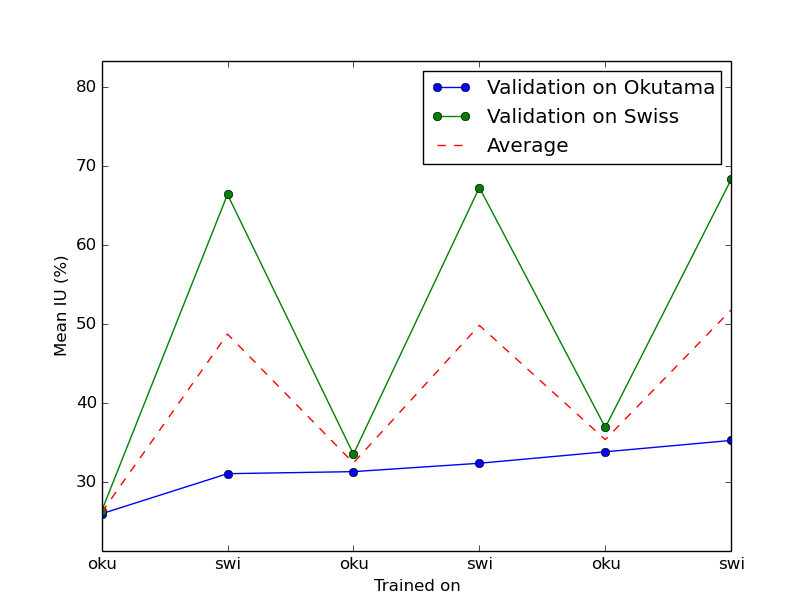
\includegraphics[width=0.8\linewidth,center]{images/part4/ms_1.png}
  \caption{Multi-source trained on baseball field images and improved on Swiss - accuracies over cycle}\textbf{
  \label{fig:part4:ms_1}}
\end{figure}

\item The second training is actually exactly the same as above, but with other data : the source dataset is now the school dataset, and the validation set is composed of the images taken from the baseball field. The Multi-source remains the same, trying to improve the results of the learning on Okutama using the Swiss dataset. The main objective of this experiment is to detect if the images from the baseball field and the ones from the school are "equivalent", that means, if they have similar influence on the learning on Okutama dataset. If we get the same results as above, it would mean that they are equivalent, and that our results are reliable. If we do not, it would mean that one of the two datasets gives more information on the other one than the second dataset on the first one. In this case, we would have to consider the lower result. \\
As shown in the graph~\ref{fig:part4:ms_2}, we notice that the results are  better in this experiment, so we can imagine that the dataset with images taken from the school includes many information concerning images taken from the baseball field. The reciprocal seems false.

\begin{figure}[ht!]
  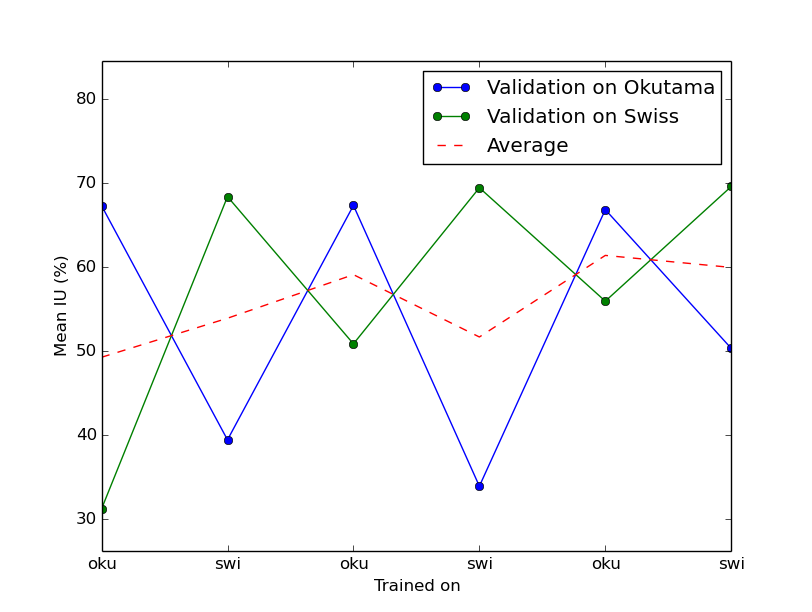
\includegraphics[width=0.8\linewidth,center]{images/part4/ms_2.png}
  \caption{Multi-source trained on school images and improved on Swiss - accuracies over cycle}\textbf{
  \label{fig:part4:ms_2}}
\end{figure}

\item The third experiment is done between the two whole datasets : we first learn features from the Okutama training set (80\%), and try to improve it with the Swiss training set (80\%). The validation set is done on the Okutama and on the Swiss validation sets, we try to improve both of them. \\
This learning shows some improvements on the Swiss dataset, but not a lot on the Okutama set, as seen above, on the first experiment. The graph~\ref{fig:part4:ms_3} shows, again, the evolution of the accuracy. 

\begin{figure}[ht!]
  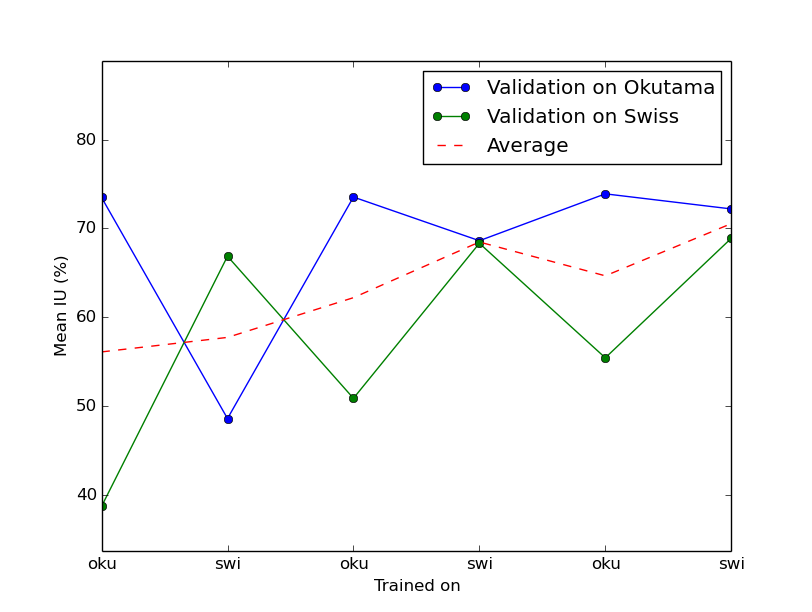
\includegraphics[width=0.8\linewidth,center]{images/part4/ms_3.png}
  \caption{Multi-source trained on Okutama images and improved on Swiss - accuracies over cycle}\textbf{
  \label{fig:part4:ms_3}}
\end{figure}

\end{enumerate}

\subsubsection{The Multi-Source utility}
So it appears that the Multi-Source method shows a real interest for merging efficiently knowledges from two different datasets into one single model, even if it does not improve the accuracy of the source dataset, at least in the case of our datasets. \\
But if we simply want to learn from these two datasets, why would we not simply train our model on all the images all at once ? We also tried this method to compare it with our multi-source method. The table~\ref{fig:part4:setup4} shows the results on both of these experiments, and shows that the accuracies from the multi-source are higher than the ones from the intuitive model. Indeed, the learning with the two different datasets try to learn features suiting to both of them, whereas the multi-source learning try to merge the knowledge on the target dataset into the pre-computed knowledge of the source dataset.

\rowcolors{2}{gray!25}{white}
\begin{table}[htbp]
  \centering
  
  \begin{tabular}{rcccccc}
  \rowcolor{gray!50}
  \toprule
   & \textbf{Train on} & \textbf{Mean IU} & \textbf{fwIU} \\
  \midrule
  Validate on Swiss & both	&		66.68			&	91.76 \\
  Validate on Swiss & ms		&		\textbf{68.87}	&	\textbf{92.52} \\
  \midrule
  Validate on Okutama & both &		68.7	0			&	77.73 \\
  Validate on Okutama & ms   &		\textbf{72.18}	&	\textbf{81.88} \\
  % last two lines switched for results
  \bottomrule
  \end{tabular}%
  
  \caption{Comparison of the data augmentation methods on both datasets.}
  \label{fig:part4:setup4}
\end{table}%

To conclude, multi-source is a good way to learn new models and include them in an other model. If we want to learn how to segment aerial urban views as well as aerial landscape views, for example, multi-source may be one of the best way to do it.


\addcontentsline{toc}{subsection}{Setup 5. Ensembles, efficiency and speed}
\subsection*{Setup 5. Ensembles, efficiency and speed}
Few studies~\cite{MARM16} \todo{find an other one} proves the efficiency of the ensembles method, that means computing few different architectures on the same dataset and, then, averaging their output in a given way. This method is really heavy, and we also need to distillate our result to get a faster (altered) model. The main objective of this part is to see if it is possible to get better results with an altered ensemble than with single models.

The results of our ensembles are shown in the table~\ref{part4:setup5:ensembles}. We can see that we are able to improve our results on our architecture, but it considerably increases the processing time. The table~\ref{part4:setup5:distillated} shows the same ensembles, but with the distillation process which drastically decreases the processing time but also a bit the accuracy. The last table (~\ref{part4:setup5:comp}) simply shows the comparison of the architectures of the ensemble alone with their respective distillated ensembles. It appears that we are not able to improves the accuracy (while keeping the same processing time) using this way, because the distillated ensembles finally appears to provide lower accuracies. Some additional tests may be relevant here, considering that we tried the same technique on an other dataset (Pascal VOC) with success, as shown in the table \todo{add ref} in the appendices.
\todo{redo this table}

\todo{replicate everything}
% from array 1 : 3, 4 are false
% from array 2 : eveything is false
\rowcolors{2}{gray!25}{white}
\begin{table}[ht!]
  
  \begin{subtable}{\textwidth}
    \centering
    \begin{tabular}{cccccc}
    \rowcolor{gray!50}
    \toprule
    \textbf{Name} & \textbf{Mean IU} & \textbf{fwIU} & \textbf{Processing time / img}\\
    \midrule
    1	& 68.43				& 81.13				& 0.37 \\
    2	& 70.41				& 80.11				& 0.37 \\
    3	& \textbf{70.87}		& \textbf{81.15}		& 0.75 \\
    4	& 68.12				& 79.04				& 0.86 \\
    \bottomrule
    \end{tabular}%
    \caption{Experiments for the setup 5 - Ensembles}
    \label{part4:setup5:ensembles}
  \end{subtable}
  
  
  \begin{subtable}{\textwidth}
    \centering
    \begin{tabular}{cccccc}
    \rowcolor{gray!50}
    \toprule
    \textbf{Name} & \textbf{Mean IU} & \textbf{fwIU} & \textbf{Processing time / img} \\
    \midrule
    1	& 66.13				& 78.24				& 0.11 \\
    2	& 69.75				& 78.11				& 0.11 \\
    3	& \textbf{67.02}		& \textbf{80.56}		& 0.12 \\
    4	& 66.62				& 79.04				& 0.11 \\
    \bottomrule
    \end{tabular}%
    \caption{Experiments for the setup 5 - Distillated ensembles}
    \label{part4:setup5:distillated}
  \end{subtable}
  
  \caption{Setup 5}
\end{table}%
\label{part4:setup5}

\todo{add and replicate}
% Everything from distill ens is false
\rowcolors{2}{gray!25}{white}
\begin{table}[htbp]
  \centering
  
  \begin{tabular}{rcccccc}
  \rowcolor{gray!50}
  \toprule
  \textbf{Architecture} & \textbf{Mean IU} & \textbf{fwIU} & \textbf{Processing time / img}\\
  \midrule
  FCN-32-ResNet-50	& 64.90			& 78.0			& 0.11 \\
  FCN-32-ResNet-152	& 67.92			& 80.84			& 0.25 \\
  Distill. ens n°1	& 66.13			& 78.24			& 0.11 \\
  \midrule
  FCN-16-ResNet-50	& 71.10			& \textbf{81.33}	& 0.12 \\
  FCN-16-ResNet-152	& \textbf{72.06}	& \textbf{81.33}	& 0.25 \\
  Distill. ens n°2	& 69.75			& 78.11			& 0.11 \\
  \midrule
  Distill. ens n°3	& 67.02			& 80.56			& 0.12 \\
  \midrule
  FCN-8				& 70.15			& 79.84			& 0.22 \\
  Distill. ens n°4	& 66.62			& 79.04			& 0.11 \\
  \bottomrule
  \end{tabular}%
  \caption{Experiments for the setup 5 - Comparison}
  \label{part4:setup5:comp}

\end{table}%


\section{Final model visualization}
In the previous section, we finally saw many numbers and talked a lot about the accuracy of our models, but we never displayed the visual results.

The figure~\ref{fig:part4:visu_archi} shows some example of the results we get on both datasets for FCN8, FCN-(32/16)-ResNet-152, and with or without data augmentation. We can see, from top to bottom, the improvement of the model accuracy.

\begin{figure}[ht!]
  \centering
  \begin{subfigure}[c]{0.20\textwidth}
    \centering 
  \end{subfigure}
  \begin{subfigure}[c]{0.33\textwidth}
    \centering Swiss
  \end{subfigure}
  \begin{subfigure}[c]{0.45\textwidth}
    \centering Okutama
  \end{subfigure}
  \vspace{0.2cm}
  
  \begin{subfigure}[c]{0.20\textwidth}
    \centering Test samples
  \end{subfigure}
  \begin{subfigure}[c]{0.33\textwidth}
    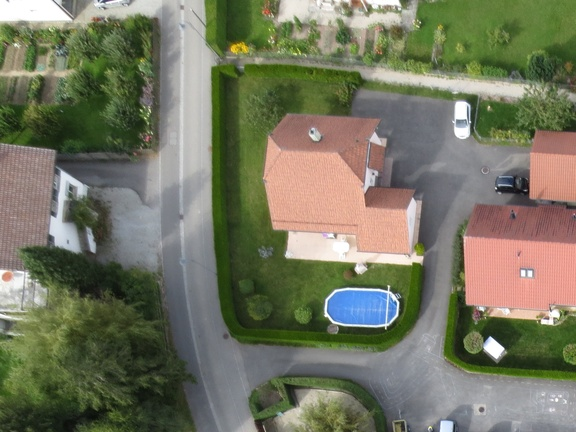
\includegraphics[height=3cm]{images/part4/swi_img.png}
  \end{subfigure}
  \begin{subfigure}[c]{0.45\textwidth}
    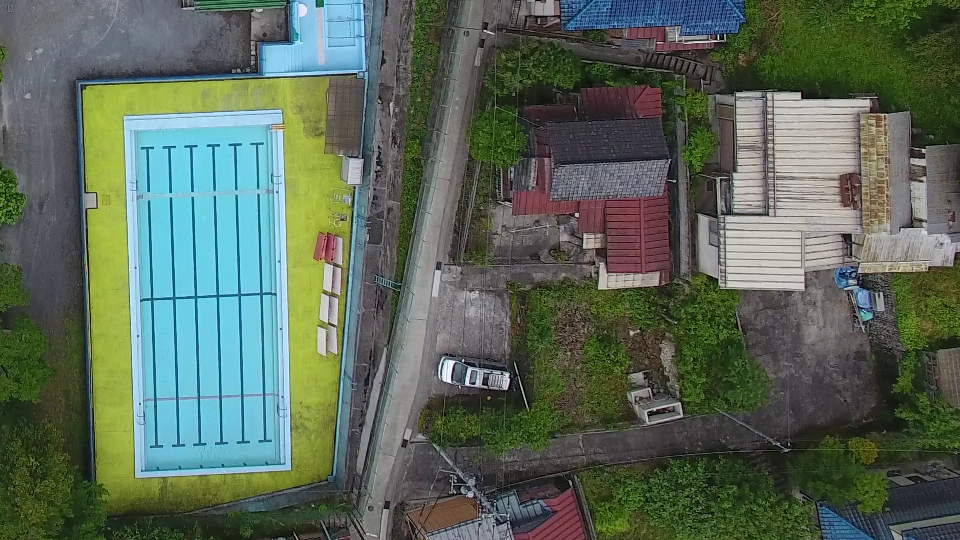
\includegraphics[height=3cm]{images/part4/oku_img.png}
  \end{subfigure}
  \vspace{0.1cm}
  
  \begin{subfigure}[c]{0.20\textwidth}
    \centering Ground truth
  \end{subfigure}
  \begin{subfigure}[c]{0.33\textwidth}
    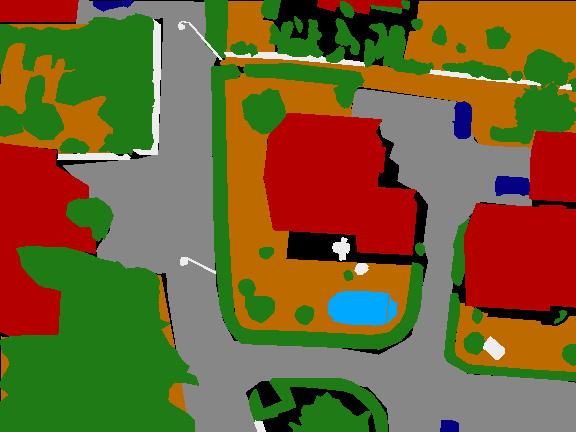
\includegraphics[height=3cm]{images/part4/swi_gt.png}
  \end{subfigure}
  \begin{subfigure}[c]{0.45\textwidth}
    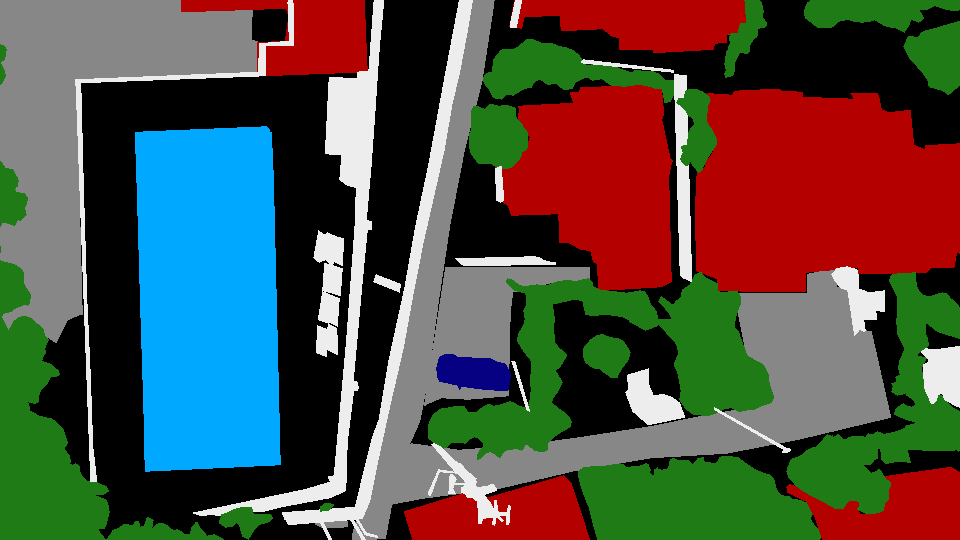
\includegraphics[height=3cm]{images/part4/oku_gt.png}
  \end{subfigure}
  \vspace{0.1cm}
  
  \begin{subfigure}[c]{0.20\textwidth}
    \centering FCN-8
  \end{subfigure}
  \begin{subfigure}[c]{0.33\textwidth}
    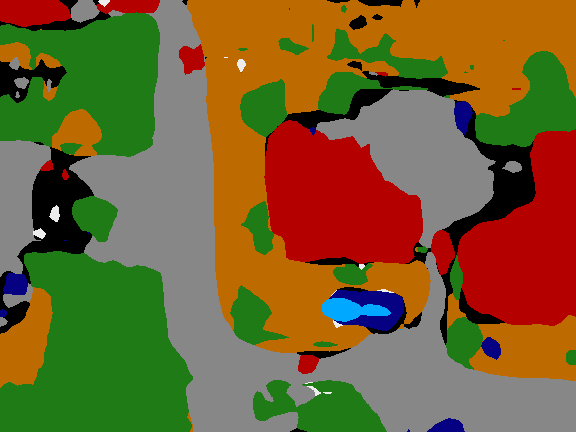
\includegraphics[height=3cm]{images/part4/swi_fcn8.png}
  \end{subfigure}
  \begin{subfigure}[c]{0.45\textwidth}
    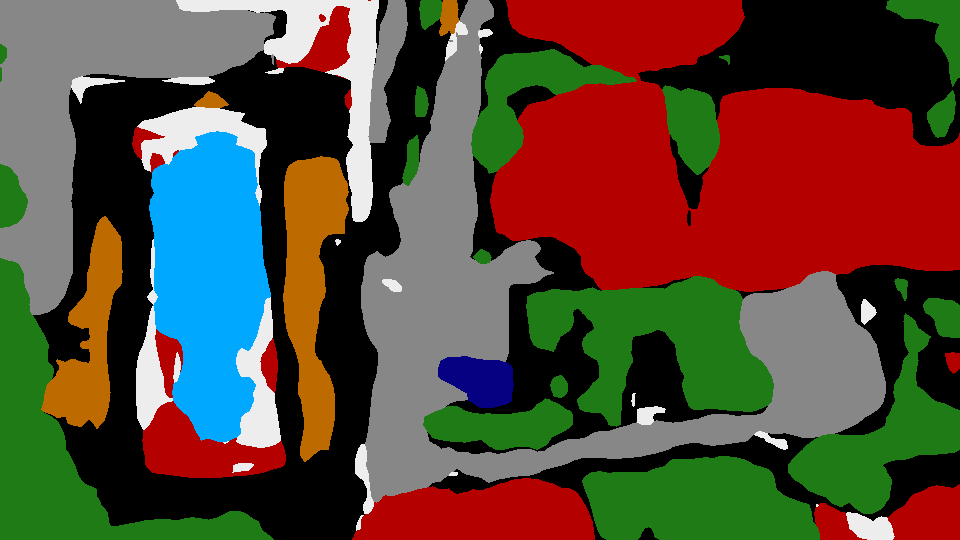
\includegraphics[height=3cm]{images/part4/oku_fcn8.png}
  \end{subfigure}
  \vspace{0.1cm}
  
  \begin{subfigure}[c]{0.20\textwidth}
    \centering FCN-32-ResNet-152
  \end{subfigure}
  \begin{subfigure}[c]{0.33\textwidth}
    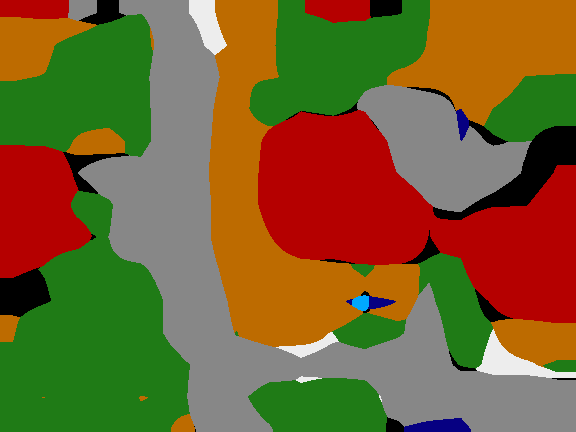
\includegraphics[height=3cm]{images/part4/swi_152.png}
  \end{subfigure}
  \begin{subfigure}[c]{0.45\textwidth}
    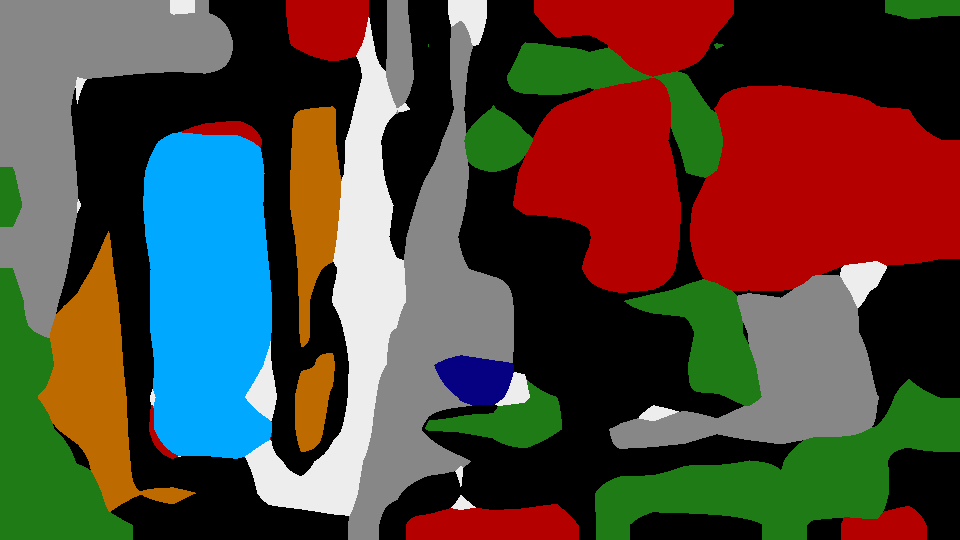
\includegraphics[height=3cm]{images/part4/oku_152.png}
  \end{subfigure}
  \vspace{0.1cm}
  
  \begin{subfigure}[c]{0.20\textwidth}
    \centering FCN-16-ResNet-152
  \end{subfigure}
  \begin{subfigure}[c]{0.33\textwidth}
    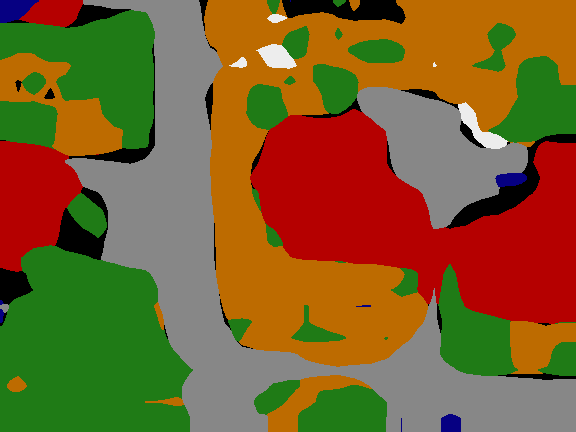
\includegraphics[height=3cm]{images/part4/swi_152s.png}
  \end{subfigure}
  \begin{subfigure}[c]{0.45\textwidth}
    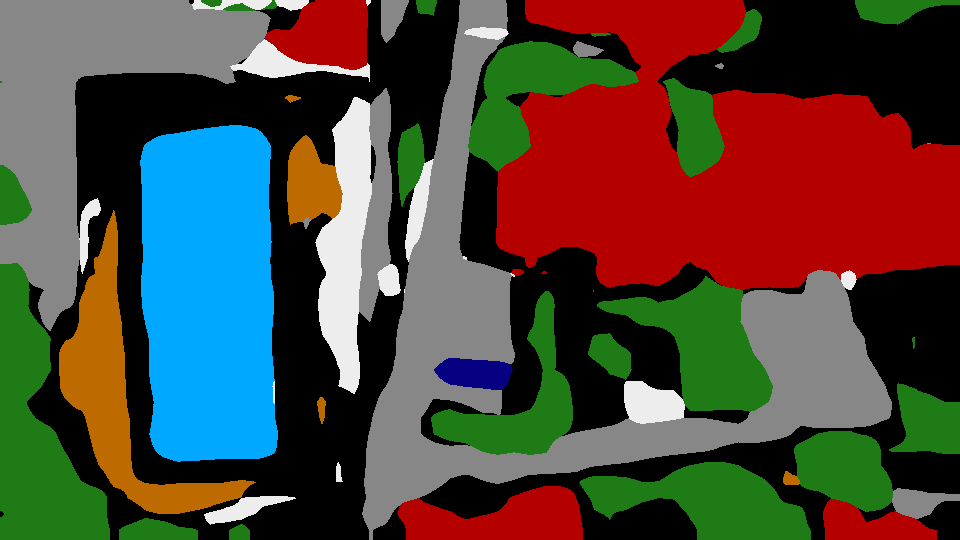
\includegraphics[height=3cm]{images/part4/oku_152s.png}
  \end{subfigure}
  \vspace{0.1cm}
  
  \begin{subfigure}[c]{0.20\textwidth}
    \centering + Mirror (data augmentation)
  \end{subfigure}
  \begin{subfigure}[c]{0.33\textwidth}
    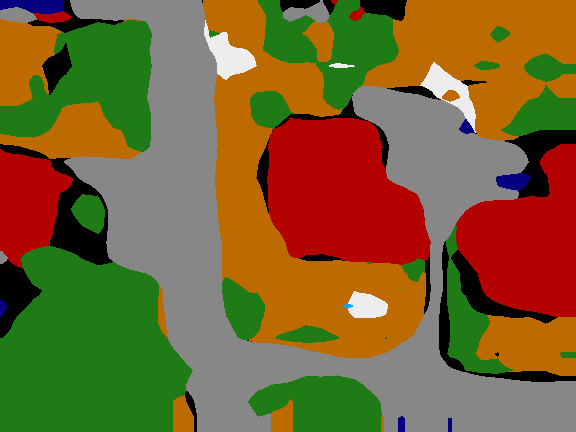
\includegraphics[height=3cm]{images/part4/swi_mirror.png}
  \end{subfigure}
  \begin{subfigure}[c]{0.45\textwidth}
    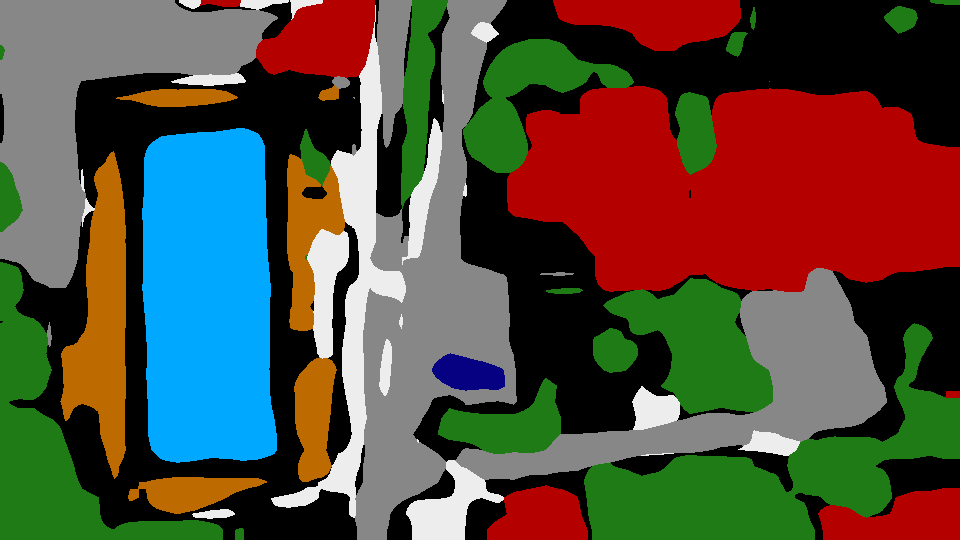
\includegraphics[height=3cm]{images/part4/oku_mirror.png}
  \end{subfigure}
  \vspace{0.1cm}
  
  \caption{Visualization of the performance over architectures and datasets}
\end{figure}
\label{fig:part4:visu_archi}

Also, the figure~\ref{fig:part4:visu_ms} shows an example of the improvement we get using Multi-Source method. This specific example consists in training our architecture on the Okutama dataset and, then, to improve it by training it on the Swiss dataset (last experiment on section~\ref{3:setups:4}). We can clearly see the accuracy improvement on the Swiss validation with the multi-source method, and also can notice that our system is still able to provide a good segmentation on the Okutama dataset. Also, we can compare our segmentations with the segmentations we get by training both datasets all at once, and the multi-source's clearly provide better results.

\begin{figure}[ht!]
  \centering
  \begin{subfigure}[c]{0.20\textwidth}
    \centering 
  \end{subfigure}
  \begin{subfigure}[c]{0.33\textwidth}
    \centering Swiss (Target)
  \end{subfigure}
  \begin{subfigure}[c]{0.45\textwidth}
    \centering Okutama (Source)
  \end{subfigure}
  \vspace{0.2cm}
  
  \begin{subfigure}[c]{0.20\textwidth}
    \centering Test samples
  \end{subfigure}
  \begin{subfigure}[c]{0.33\textwidth}
    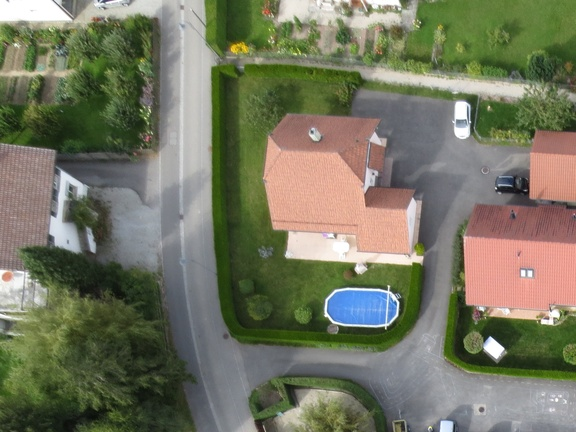
\includegraphics[height=3cm]{images/part4/swi_img.png}
  \end{subfigure}
  \begin{subfigure}[c]{0.45\textwidth}
    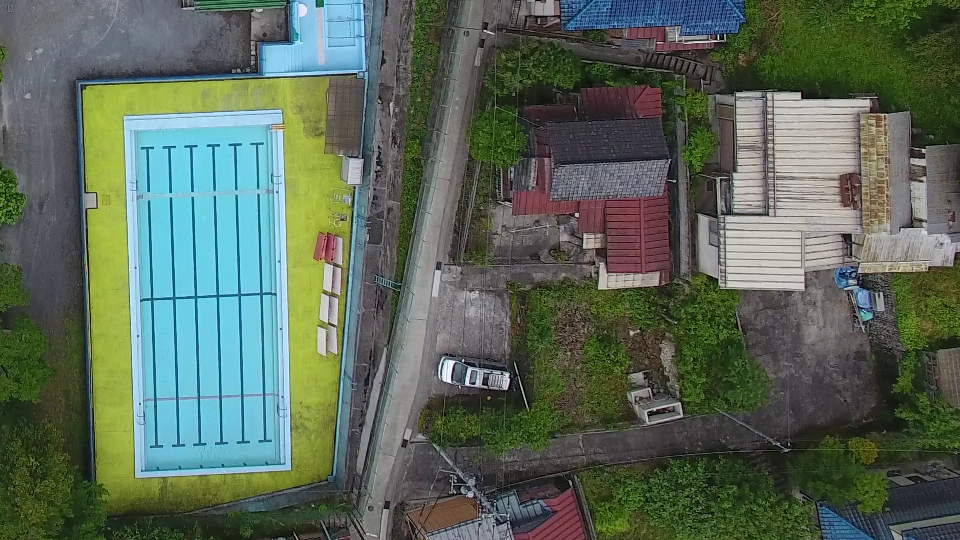
\includegraphics[height=3cm]{images/part4/oku_img.png}
  \end{subfigure}
  \vspace{0.1cm}
  
  \begin{subfigure}[c]{0.20\textwidth}
    \centering Ground truth
  \end{subfigure}
  \begin{subfigure}[c]{0.33\textwidth}
    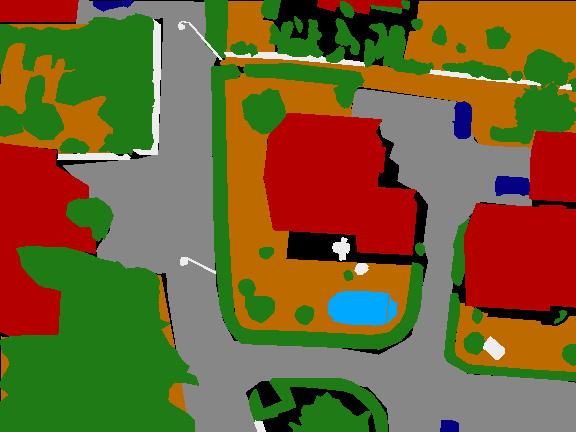
\includegraphics[height=3cm]{images/part4/swi_gt.png}
  \end{subfigure}
  \begin{subfigure}[c]{0.45\textwidth}
    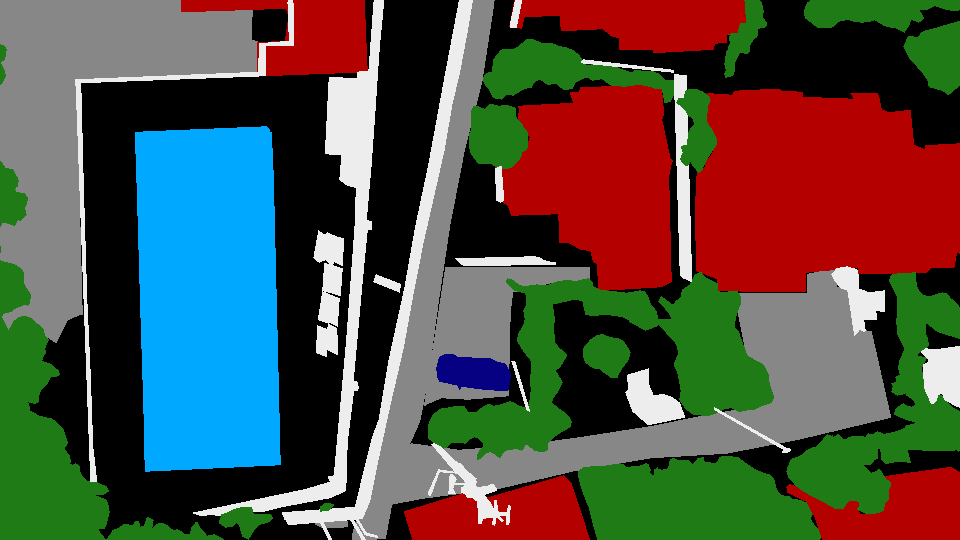
\includegraphics[height=3cm]{images/part4/oku_gt.png}
  \end{subfigure}
  \vspace{0.3cm}
  
  \begin{subfigure}[c]{0.20\textwidth}
    \centering Train both datasets together
  \end{subfigure}
  \begin{subfigure}[c]{0.33\textwidth}
    %\includegraphics[height=3cm]{images/part4/swi_allatonce.png}
    \centering Missing swi\_allatonce.png
  \end{subfigure}
  \begin{subfigure}[c]{0.45\textwidth}
    %\includegraphics[height=3cm]{images/part4/oku_allatonce.png}
    \centering Missing oku\_allatonce.png
  \end{subfigure}
  \vspace{0.3cm}
  
  \begin{subfigure}[c]{0.20\textwidth}
    \centering Train Okutama alone
  \end{subfigure}
  \begin{subfigure}[c]{0.33\textwidth}
    %\includegraphics[height=3cm]{images/part4/swi_okualone.png}
    \centering Missing swi\_okualone.png
  \end{subfigure}
  \begin{subfigure}[c]{0.45\textwidth}
    %\includegraphics[height=3cm]{images/part4/oku_okualone.png}
    \centering Missing oku\_okualone.png
  \end{subfigure}
  \vspace{0.1cm}
  
  \begin{subfigure}[c]{0.20\textwidth}
    \centering Multi-source from Okutama to Swiss
  \end{subfigure}
  \begin{subfigure}[c]{0.33\textwidth}
    %\includegraphics[height=3cm]{images/part4/swi_okutransfered.png}
    \centering Missing swi\_okutransfered.png
  \end{subfigure}
  \begin{subfigure}[c]{0.45\textwidth}
    %\includegraphics[height=3cm]{images/part4/oku_okutransfered.png}
    \centering Missing oku\_okutransfered.png
  \end{subfigure}
  \vspace{0.1cm}
  
  \caption{Visualization of the multi-source method efficiency}
  \label{fig:part4:visu_ms}
\end{figure}

A video example of this work can also be viewed on YouTube, at the following link : https://youtu.be/X73HLjDhtKU.



\section{Test on real device}
We have defined a good architecture for semantic segmentation on aerial views and we, now, want to use it on real situations, that means to implement it in our drone to see if the accuracy and speed would be good enough on a small device (and not anymore on a powerful server).

The implementation will be done on a 64-bit ARM\textregistered A57 CPU, that will run the DL architecture \textit{via} Caffe on the Jetson TX1 GPU~\footnote{nvidia.com/object/jetson-tx1-module}, from Nvidia. These devices are handled by the Phantom drone from DJI~\footnote{dji.com/jp/product/phantom} that captures images of size 3840x2160 with a 4K GoPro.

It appears that the speed of our architecture considerably decreased when it is implemented in the drone : we have a result closer to one frame per second (1FPS) instead of 10FPS on the server. The 1FPS is still acceptable for applications in quite real-time, but would not be enough for more complicated tasks, considering that the understanding of the scene is not everything, we would still want to implement some action algorithms, depending on the understood situations. It may takes some additional time, require a free GPU, and the 1FPS may quickly be a strong limitation.

A first solution would be to process smaller images (ours are high definition, this is quite big and probably not that useful). Cropping the image into a medium field-of-view will accelerate the processing time. Moreover, this operation can be done directly from the camera, to avoid images pre-processing time. However, it also will decrease the understanding of the scene : the drone would segment the really "in front" scene, and would not have a understanding on a large field of view as before.

A second solution would be to optimize our code, currently wrote in Python, and maybe to convert it into C++, which is much weaker. However, we have to admit that our code already use some really optimized libraries (\textit{numpy}, \textit{scipy}, ...), and the conversion of our code into C++ may provide only a slight improvement.

Currently, our project is frozen there, we try to find some other ways to decrease the computational needs on the drone, and to provide a real-time application.



